\def\mytitle{AVR-GCC ASSIGNMENT}
\def\myauthor{koushik kalyani}
\def\mycontact{koushikkalyani369@gmail.com}
\def\mymodule{Future Wireless Communication}
\documentclass[journal,12pt,twocolumn]{IEEEtran}
\usepackage{graphicx} 
\usepackage{enumitem}
\usepackage{tikz}
\usepackage{circuitikz}
\usepackage{karnaugh-map}
\usepackage{tabularx}
\title{\mytitle}
\author{\myauthor\\\mycontact\\IITH\hspace{0.3em}-\hspace{0.3em}\mymodule}
\begin{document}
\maketitle
\tableofcontents

\section{\textbf{Question}}
The output $F$ of the digital circuit shown can be written in form(s) \rule{12mm}{0.6pt}
\vspace{\baselineskip}\\
\resizebox{0.45\textwidth}{!}{
\begin{tikzpicture}

  % First Mux
  \draw (0,0) rectangle (2,2);
  \draw (1,0) -- (1,-1);
  \draw (2,1) -- (3,1);
  \node at (0.5,1.5) {$I_0$};
  \node at (0.5,0.5) {$I_1$};
  \node at (2.5,1.3) {Y};
  \node at (1.25,-1) {B};
  \draw(3,1) |-(4,0.52);
  % Second Mux
  \draw (4,0) rectangle (6,2);
  \draw (5,0) -- (5,-1);
  \node at (4.5,1.5) {$I_0$};
  \node at (4.5,0.5) {$I_1$};
  \node at (5.25,-1) {A};
 \draw(0,1.55)--(-0.75,1.55);
 \draw(0,0.55)--(-0.75,0.55);
 \draw(4,1.55)--(3.25,1.55);
 \node at (-1,1.55){$1$};
  \node at (-1,0.55){$0$};
  \node at (3,1.55){$1$};
  \draw[->] (6,1) -- (7,1);
  \node at (7.5,1) {F};
\end{tikzpicture}}
\begin{enumerate}[label=(\alph*)]
    \item $\overline{A \cdot B} $
    \item $\overline A + \overline B$
    \item $ \overline{A+B}$
    \item $\overline A \cdot \overline B$
\end{enumerate}
    \section{\textbf{Answer}}
    The above question can reduced as follows \\
    $\rightarrow Y=\bar B\cdot 1 + B \cdot 0$
    $\rightarrow Y=\bar B$\\
    $\rightarrow F = \bar A \cdot 1 + A \cdot \bar B$
    $\rightarrow F = (\bar A + A)\cdot(\bar A+ \bar B)$\\
    $\rightarrow F = \bar A + \bar B$ also $F=\overline{A\cdot B}$\\
    Therefore, the Boolean function $F = \bar A + \bar B$
   \section{\textbf{Logic Diagram}}
   \begin{center} 
   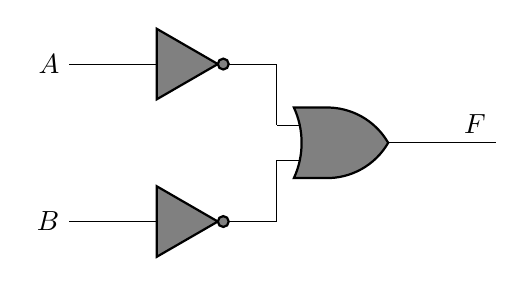
\begin{tikzpicture}
\ctikzset{
    logic ports=ieee,
    logic ports/scale=0.8,
    logic ports/fill=gray
}
% Logic ports
\node[not port] (notx) at (1,0){};
\node[not port]  (notz) at (1,-2){};
\node[or port] (orf) at (3,-1){};
\draw(notx.out)-|(orf.in 1);
 \draw(notz.out)-|(orf.in 2);
\draw(orf.out)-- ++(1.05,0) node[near end,above]{$F$};
 \draw(notz.in)-- ++(-0.8,0) node[left]{$B$};
 \draw(notx.in)-- ++(-0.8,0) node[left]{$A$};
\end{tikzpicture}
\begin{center}
Fig. 1 
\end{center}
       \end{center}
           \section{\textbf{Truth Table}}
\begin{tabularx}{0.45\textwidth}{
  | >{\centering\arraybackslash}X  
  | >{\centering\arraybackslash}X 
  | >{\centering\arraybackslash}X |
  }
  \hline
  \textbf{$A$}&\textbf{$B$}&\textbf{$F$}\\
  \hline
  0&0&1\\
  \hline
  0&1&1\\
  \hline
  1&0&1\\
  \hline
  1&1&0\\
  \hline
  \end{tabularx}
     \begin{center}
 Truth table for Boolean Function $F$
\end{center}
    \section{\textbf{K-Map Implementation}}
    Using the boolean logic output $F$ can be expressed in terms of the inputs $A,B$ with the help of the following K-map.
    \begin{center}
      \resizebox{0.45\textwidth}{!}{%
      \begin{karnaugh-map}[2][2][1][$B$][$A$]
            \maxterms{3}
            \minterms{0,1,2}
            \implicant{0}{1}
            \implicant{0}{2}
        \end{karnaugh-map}%
        }
    \end{center}
    \begin{center}
Fig. 2
\end{center}
\begin{center}
    \section{\textbf{Components}}
  \begin{tabularx}{0.45\textwidth} { 
  | >{\centering\arraybackslash}X 
  | >{\centering\arraybackslash}X 
  | >{\centering\arraybackslash}X
  | >{\centering\arraybackslash}X | }
\hline
 \textbf{Component}& \textbf{Values} & \textbf{Quantity}\\
\hline
Arduino & UNO & 1 \\  
\hline
Jumper Wires& M-M & 4 \\ 
\hline
Breadboard &  & 1 \\
\hline
\end{tabularx}
\end{center}
\begin{center}
    \section{\textbf{Implementation}}
  \begin{tabularx}{0.46\textwidth} { 
  | >{\centering\arraybackslash}X 
  | >{\centering\arraybackslash}X 
  | >{\centering\arraybackslash}X  | }
\hline
\textbf{Arduino PIN} & \textbf{INPUT} & \textbf{OUTPUT} \\ 
\hline
\textbf 2 & A & \\
\hline
\textbf 3 & B & \\
\hline
\textbf	{13}& & F \\
\hline
\end{tabularx}
\end{center}
\begin{center}
    Connections
\end{center}
\textbf{Procedure}\\
1. Connect the circuit as per the above table.\\
2. Connect inputs to Vcc for logic 1, ground for logic 0.\\
3. Execute the circuit using the below code.\\
\\\begin{tabularx}{0.45\textwidth} { 
  | >{\centering\arraybackslash}X |
 }
  \hline
https://github.com/koushikkalyani/FWC/blob\\/main/AVR-GCC/avr.c\\
  \hline
\end{tabularx}\\
\\4. Change the values of A,B in the hardware and verify the Truth Table.\\
\end{document}
